\section*{Chapter 1}

\begin{hwproblem}
{2}{
    \text { Write out a complete Cayley table for } \(D_3\) \text {. Is } \(D_3\) \text { Abelian?}
} 

Let \(R_{d}\) be the motion of rotating the triangle by \(d\) degrees, \(V\) be the flip the triangle down the middle, \(D\) be the flip along its main diagonal, and \(D'\) the flip along its alternative diagonal.

\begin{center}
    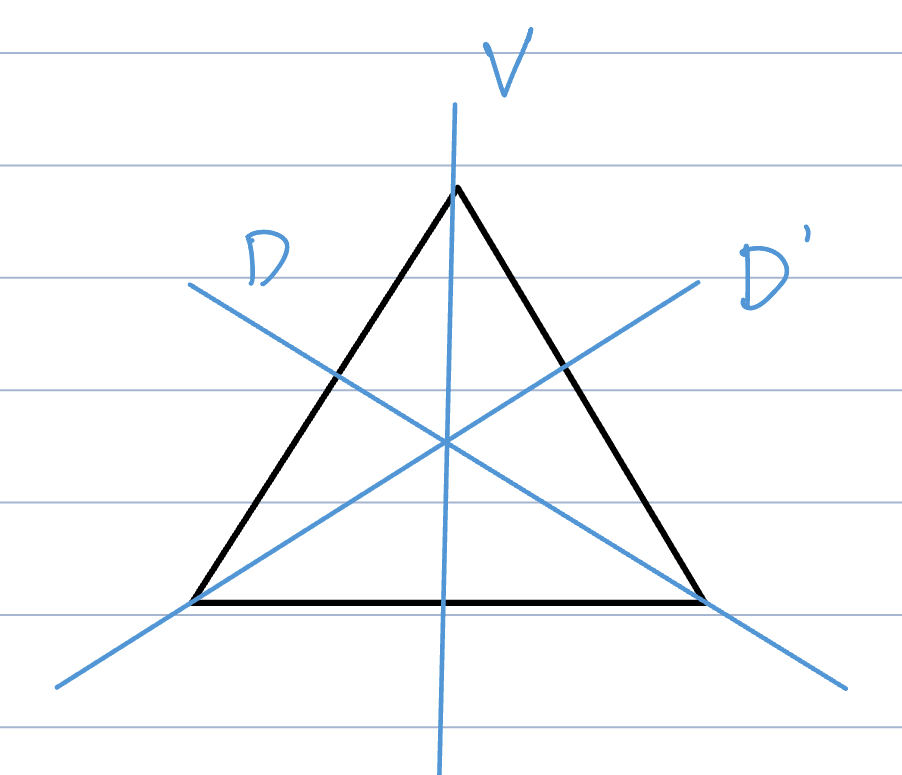
\includegraphics[width=0.4\textwidth]{images/d3-motions.jpg}
\end{center}

The table can be constructed as follows.
\begin{center}
    \begin{tabular}{|L|LLLLLL|}
        \hline
        & R_0 & R_{120} & R_{240} & V & D & D' \\
        \hline
        R_0 & R_0 & R_{120} & R_{240} & V & D & D' \\
        R_{120} & R_{120} & R_{240} & R_0 & D & D' & V \\
        R_{240} & R_{240} & R_0 & R_{120} & D' & V & D \\
        V & V & D' & D & R_0 & R_{240} & R_{120} \\
        D & D & V & D' & R_{120} & R_0 & R_{240} \\
        D' & D' & D & V & R_{240} & R_{120} & R_0 \\
        \hline
    \end{tabular}
\end{center}

Observe that \(D_3\) is non-Abelian. An example of a pair of elements that violates the commutative condition is
\[
    DV = R_{240} \neq VD = R_{120}
\]
\end{hwproblem}

\begin{hwproblem}
{6}{
    In \(D_n\), explain geometrically why a reflection followed by a reflection must be a rotation.
}

Suppose that we can identify the corners of a dihedral in \(D_n\) using integers \(1, 2, \ldots, n\). Without loss of generality, assume that we start in a configuration that the orientation of corners \(1, 2, \ldots, n\) is clockwise. When we perform the first reflection, it flips the dihedral along a line and the orientation of corners \(1, 2, \ldots, n\) will now be counter-clockwise.

Consider a pair of corners---denoted corner 1 and 2---and, without loss of generality, suppose that corner 2 lies to the right of corner 1 and corner 1 is closer to the line of reflection, the reflection will make it so that corner one is still closer to the line of reflection.
\begin{center}
    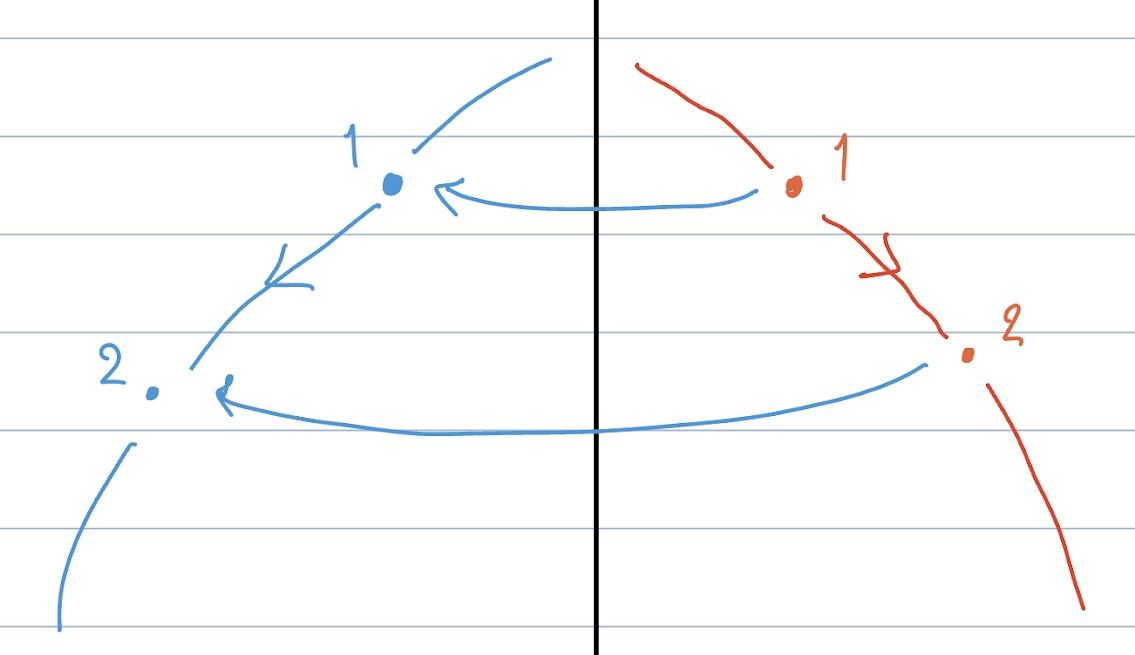
\includegraphics[width=0.5\textwidth]{images/reflection.jpg}
\end{center}
Repeating the reflection will make the orientation clockwise again and any difference in location from the original state can be achieved by a rotation. Thus, a reflection followed by a reflection must be a rotation.
\end{hwproblem}

\begin{hwproblem}
{8}{
    In \(D_n\), explain geometrically why a rotation followed by a reflection must be a reflection.
}

Assume to the contrary that a rotation followed by a reflection is a rotation. This means that we are able to fix a point and rotate the dihedral around that point to achieve the composition of rotation-then-reflection and the other way around. However, since the reflection fixes a line and reflects its corners around that line, it causes the orientation of the corners of the dihedral to be opposite of the original and no rotation move can achieve that. Thus, a rotation followed by a reflection must be a reflection.
\end{hwproblem}

\begin{hwproblem}
{10}{
    If $r_1, r_2$, and $r_3$ represent rotations from $D_n$ and $f_1, f_2$, and $f_3$ represent reflections from $D_n$, determine whether $r_1 r_2 f_1 r_3 f_2 f_3 r_3$ is a rotation or a reflection.
}

It is a reflection. The breakdown is as follows:
\begin{enumerate}
    \item \(r_1 r_2\) is a rotation, denote as \(R_1\)
    \item \(R_1 f_1\) is a reflection, denote as \(F_1\)
    \item \(F_1 r_3\) is a reflection, denote as \(F_2\)
    \item \(F_2 f_2\) is a rotation, denote as \(R_2\)
    \item \(R_2 f_3\) is a reflection, denote as \(F_3\)
    \item \(F_3 r_3\) is a reflection, so the entire composition is a reflection
\end{enumerate}
\end{hwproblem}

\begin{hwproblem}
{18}{
    Consider an infinitely long strip of equally spaced H's:
    $$\cdots\ H\ H\ H\ H\ \cdots$$
    Describe the symmetries of this strip. Is the group of symmetries of the strip Abelian?
}

This strip has symmetries: \(R_0, R_{180}, V, \text{ and } H\). For \(R_{180}\) and \(H\), since the strip goes on infinitely, it doesn't matter where you choose the axis to be since anywhere you cut the strip, the length of each sides will still be infinity.
\end{hwproblem}
